\section{Text2Process}
\begin{wrapfigure}{r}{7cm}
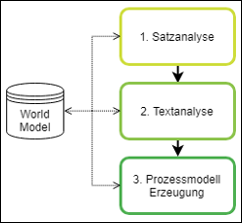
\includegraphics[width=7cm]{pictures/T2P_highlevel.png}
\caption{Vorgehen bei T2P in Anlehnung an Friedrich}
\label{fig:T2PHL}
\end{wrapfigure}
Die Umwandlung einer informellen Beschreibung eines Geschäftsprozesses in natürlicher Sprache in ein formales Prozessmodell stellt bei \ac{BPM}, wie in Kapitel 1 dargelegt, ein häufig auftretendes Problem dar. 
Der Begriff \ac{T2P} soll im Folgenden die softwaregestützte Automatisierung derartiger \ac{BPM} Umwandlungen unter Anwendung von \ac{NLP} bezeichnen.\par
Zur Realisierung von \ac{T2P} kann ein aus 3 sequentiellen Phasen bestehendes Vorgehen zur Textanalyse gewählt werden, welches von verschiedenen \ac{NLP} Tools Gebrauch macht und in Abbildung \ref{fig:T2PHL} schematisch dargestellt wird. Die einzelnen Phasen fügen dabei bezüglich des angestrebten Prozessmodels extrahierte Information inkrementell zu einer übergeordneten Datenstruktur, dem World Model, hinzu.\par
In der ersten Phase des Vorgehens werden zunächst die einzelnen Sätze im Detail analysiert. Dabei werden die grundlegenden Elemente des Prozesses ermittelt, wie etwa Akteure, Ressourcen oder Aktionen. Daraufhin wird in der zweiten Phase noch einmal der Text in seiner Gesamtheit analysiert, um auch Bezüge und Beziehungen zwischen Sätzen auswerten zu können. Im Fokus stehen nun aus Prozesssicht relevante semantische Details, wie etwa die zeitliche Abfolge der in den Sätzen beschriebenen Aktionen. Im dritten Schritt wird letztlich die finale Transformation in ein syntaktisch korrektes Prozessmodel vorgenommen. So werden etwa  eventuell entstandene Redundanzen bzw. syntaktische Unvollständigkeiten beseitigt. 


\begin{itemize} 
\item Motivation für unsere Tools herausstellen? 
\item World Model nach Buch "Natural Language Processing"
\end{itemize}

Notiz von Jana: 
Motivation für die Tools ist im Prinzip, dass der Ansatz nach Friedrich den wir analysieren wollen genau diese Tools (Stanford CoreNLP, WordNet und FrameNet) nutzt (siehe Riefer et al Seite 8). Finde deshalb wirs sollten das NLTK nicht als eigenes Kapitel sondern in Stanford integriert betrachten. Außerdem wird Friedrich als State-Of-The-Art definiert (Seite 11). Kann man hier vielleicht auch erwähnen. 
